\section{Simulation Analysis and Comparison with Theoretical Results}
\label{sec:simulation}

\subsection{Operating Point Analysis}

	Table~\ref{tab1:op} shows the simulated operating point results for the circuit
under analysis for t$<$0, which means that we will consider the voltage source $v_s$ as a 
DC voltage source equal to $V_s$, given in the Python script. Notice that the values on the right
were obtained by Octave, therefore they are the theoretical values, which we already mentioned previously 
but, to facilitate the comparison between the simulation and theoretical values, we mentioned them again.

\begin{table}[H]
  \centering
  \begin{tabular}{|l|r|}
    \hline    
    {\bf Name} & {\bf Value [A or V]} \\ \hline
    @c[i] & 0.000000e+00\\ \hline
@gb[i] & -2.24935e-04\\ \hline
@r1[i] & 2.149178e-04\\ \hline
@r2[i] & -2.24935e-04\\ \hline
@r3[i] & -1.00169e-05\\ \hline
@r4[i] & 1.233378e-03\\ \hline
@r5[i] & -2.24935e-04\\ \hline
@r6[i] & 1.018460e-03\\ \hline
@r7[i] & 1.018460e-03\\ \hline
v1 & 5.248421e+00\\ \hline
v2 & 5.033187e+00\\ \hline
v3 & 4.581562e+00\\ \hline
v4 & -2.05008e+00\\ \hline
v5 & 5.064367e+00\\ \hline
v6 & 5.745178e+00\\ \hline
v7 & -2.05008e+00\\ \hline
v8 & -3.09813e+00\\ \hline

  \end{tabular}
  \begin{tabular}{|l|r|}
    \hline    
    {\bf Node} & {\bf Voltage[V]} \\ \hline
    $V_{1}$ & 1.726209e+00 \\ \hline
$V_{2}$ & -2.924287e-01 \\ \hline
$V_{3}$ & -4.528138e+00 \\ \hline
$V_{4}$ & 9.535580e+00 \\ \hline
$V_{5}$ & 9.279827e-06 \\ \hline
$V_{6}$ & -1.191502e+00 \\ \hline
$V_{7}$ & -3.522212e+00 \\ \hline

  \end{tabular}
  \begin{tabular}{|l|r|}
    \hline    
    {\bf Name} & {\bf Value [A or V]} \\ \hline
    $V_{b}$ & -2.924287e-01 \\ \hline
$I_{b}$ & -2.109620e-03 \\ \hline
$V_{c}$ & -9.279827e-06 \\ \hline
$I_{c}$ & -1.157872e-03 \\ \hline
$I_{R1}$ & -2.015673e-03 \\ \hline
$I_{R2}$ & -2.109620e-03 \\ \hline
$I_{R3}$ & -9.394704e-05 \\ \hline
$I_{R4}$ & 8.578007e-04 \\ \hline
$I_{R5}$ & 3.150480e-03 \\ \hline
$I_{R6}$ & -1.157872e-03 \\ \hline
$I_{R7}$ & -1.157872e-03 \\ \hline

  \end{tabular}
  \caption {Operating point for t<0. A variable preceded by @ is of type {\em current}
    and expressed in Ampere; other variables are of type {\it voltage} and expressed in
    Volt. The values on the right are the theoretical values for the currents and voltages in the circuit.}
  \label{tab1:op}
\end{table}


	Compared to the theoretical analysis results, we notice that both simulation results are accurate, except for the last 
decimal places, as a consequence of the cientific notation and the number of significative algharisms used by each program to 
present the results. Despite that, we realise that the values with more significant algharisms match correctly the rounded values.


	Table~\ref{tab2:op} shows the simulated operating point results for the circuit
under analysis for t=0, where we will consider the voltage source $v_s$=0 and replace the
capacitor for a voltage source $V_x$=$V_6$-$V_8$, where $V_6$ and $V_8$ are the voltages in
nodes 6 and 8, respectively. This step will allow us to verify the theoretical results obtained 
for the node voltages and the current $I_x$, which are accurate, as we can see. Again, we show
the theoretical values obtained for this step, to make it easier to compare between simulation
and theoretical values.



\begin{table}[H]
  \centering
  \begin{tabular}{|l|r|}
    \hline    
    {\bf Name} & {\bf Value [A or V]} \\ \hline
    @gb[i] & 0.000000e+00\\ \hline
@r1[i] & 0.000000e+00\\ \hline
@r2[i] & 0.000000e+00\\ \hline
@r3[i] & 0.000000e+00\\ \hline
@r4[i] & 0.000000e+00\\ \hline
@r5[i] & -2.92176e-03\\ \hline
@r6[i] & 0.000000e+00\\ \hline
@r7[i] & 0.000000e+00\\ \hline
v1 & 0.000000e+00\\ \hline
v2 & 0.000000e+00\\ \hline
v3 & 0.000000e+00\\ \hline
v4 & 0.000000e+00\\ \hline
v5 & 0.000000e+00\\ \hline
v6 & 8.843309e+00\\ \hline
v7 & 0.000000e+00\\ \hline
v8 & 0.000000e+00\\ \hline

  \end{tabular}
  \begin{tabular}{|l|r|}
    \hline    
    {\bf Name} & {\bf Value [A or V]} \\ \hline
    $V_{1}$ & 0.000000e+00 \\ \hline
$V_{2}$ & 0.000000e+00 \\ \hline
$V_{3}$ & 0.000000e+00 \\ \hline
$V_{5}$ & 0.000000e+00 \\ \hline
$V_{6}$ & 8.843309e+00 \\ \hline
$V_{7}$ & -0.000000e+00 \\ \hline
$V_{8}$ & 0.000000e+00 \\ \hline

  \end{tabular}
  \begin{tabular}{|l|r|}
    \hline    
    {\bf Name} & {\bf Value [A or V]} \\ \hline
    $V_{x}$ & 8.843309e+00 \\ \hline
$I_{x}$ & 2.921760e-03 \\ \hline
$R_{eq}$ & 3.026707e+03 \\ \hline

  \end{tabular}
  \caption{Operating point for t=0, where the capacitor $C$ was replaced by a voltage source $V_x$=$V_6$-$V_8$, with $V_6$ and $V_8$ obtained previously. 
  A variable preceded by @ is of type {\em current} and expressed in Ampere; other variables are of type {\it voltage} and expressed in Volt. The values on the right are the theoretical 
  values for the currents and voltages in the circuit.}
  \label{tab2:op}
\end{table}


Furthermore, we can see that for t$<$0, $V_6$ will have a significant different voltage value than for t=0; however, the voltage in the capacitor $C$, which is given by $V_6$-$V_8$ remains the same, despite the different values for $V_6$ and $V_8$. Therefore, we witness a discontinuity in the node voltages,
that does not happen for the voltage in the capacitor - well, this happens because only the voltages in capacitors and inductors remain continuous, therefore the voltages in the resistors will have 'jumps' in their values to mantain the continuity previously mentioned. 


In both tables, we can see a nineth node (node 4), which has the same voltage value as node 7. This happens because, in NGSPice, when we want to simulate circuits with current-dependent sources, we must add a 0V voltage source in series to a component to sense the current flowing through it. Therefore, an aditional node appears in the simulated circuit.


\subsection{Transient Analysis}


Figure~\ref{fig:trans1} shows the simulated transient analysis results for the natural response of 
the circuit under analysis, using the boundary conditions for $V_6$ and $V_8$ obtained previously
in the second operating point analysis performed. 

\begin{figure}[H] \centering
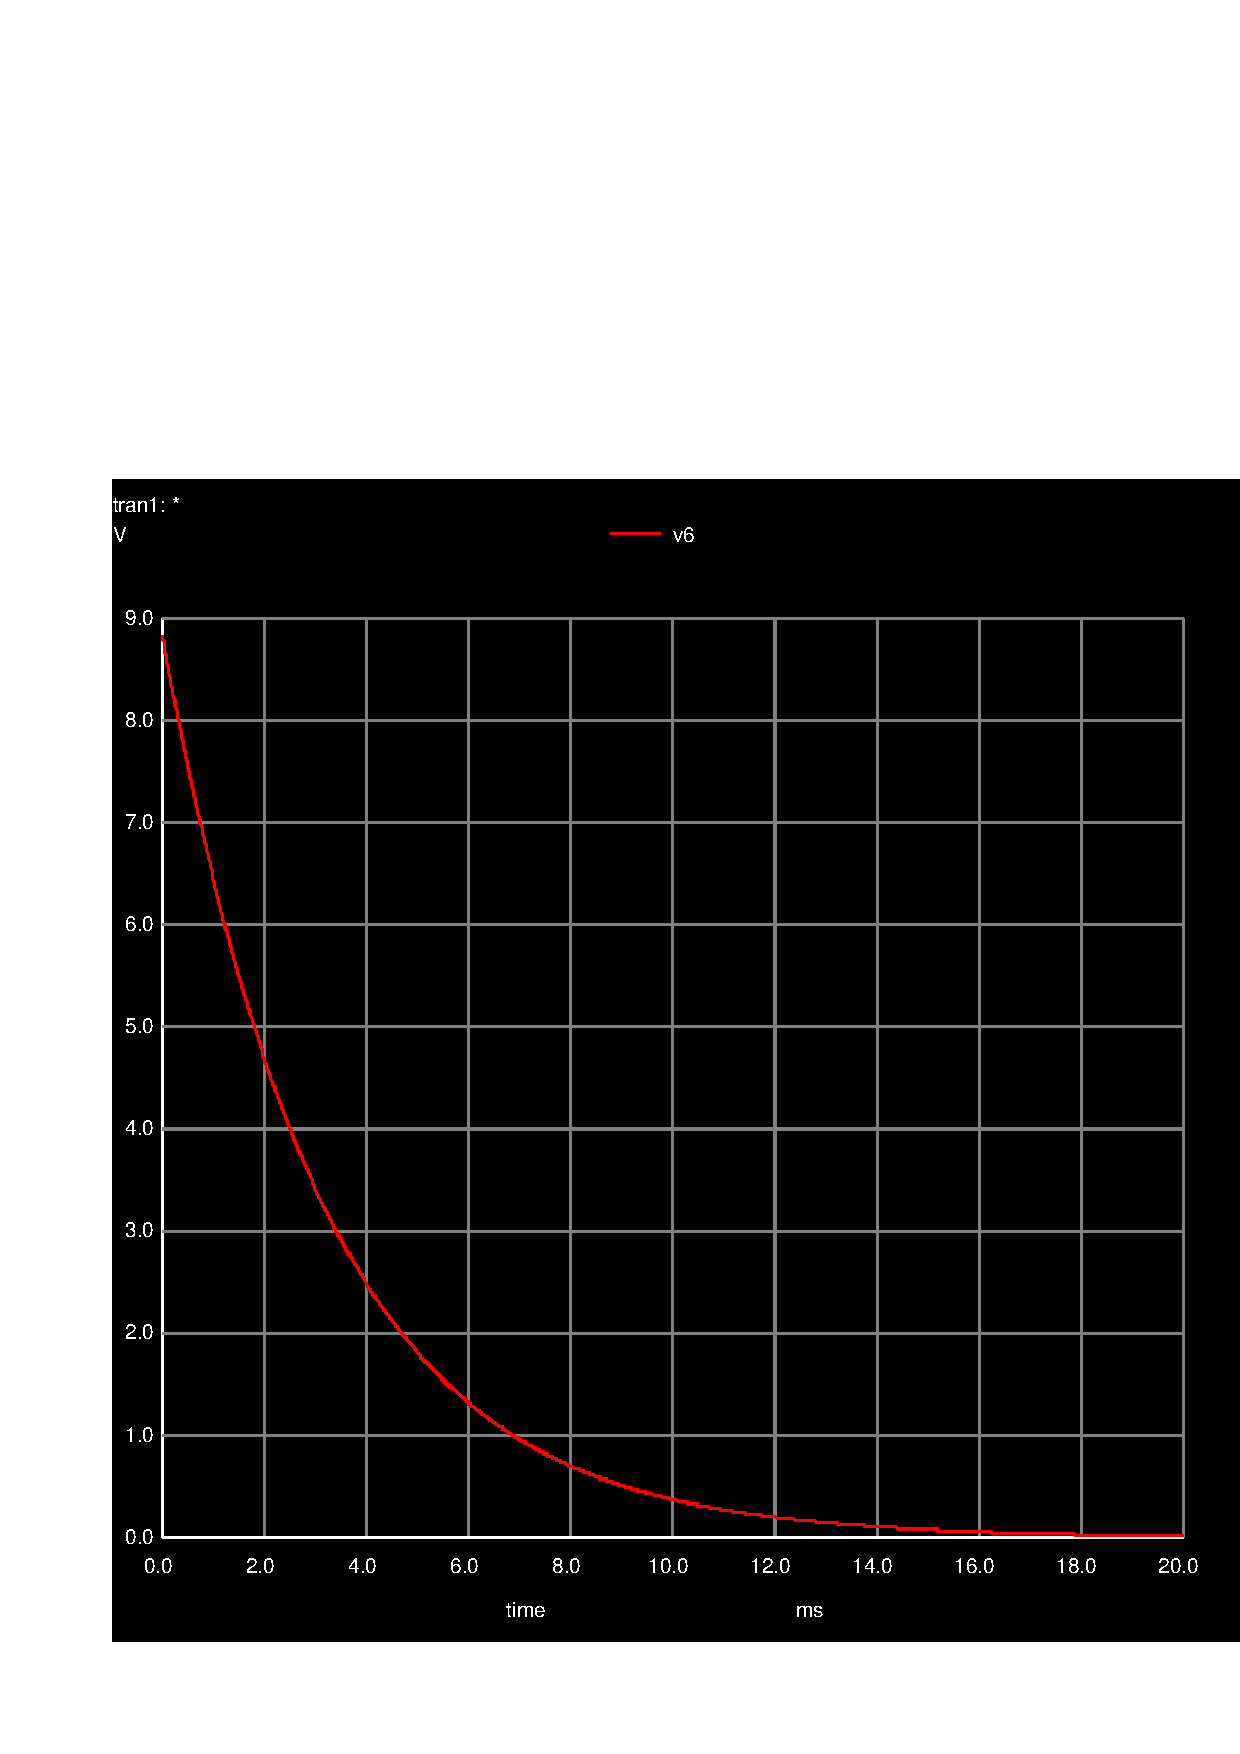
\includegraphics[width=0.4\linewidth]{trans1.pdf}
\caption{Transient output voltage for node 6, with boundary conditions $V_6$ and $V_8$ obtained previously.}
\label{fig:trans1}
\end{figure}

We can notice that the graphic for the voltage $V_6$ is in a form of a negative exponential, 
which is confirmed by the expression and respective graphic obtained for the theoretical 
analysis, performed in Octave. Furthermore, because the theoretical analysis is performed
for the interval [-5; 20]ms, we can easily notice the discontinuity for the voltage values
$v_s$ and $V_6$, that does not happen for the voltage in the capacitor.


Figure~\ref{fig:trans2} shows the simulated transient analysis results for the
circuit under analysis, where we finally consider the voltage source $v_s$,
as a sinusoidal fuction of time. We perform this simulation to obtain the total
solution (natural+forced).

\begin{figure}[H] \centering
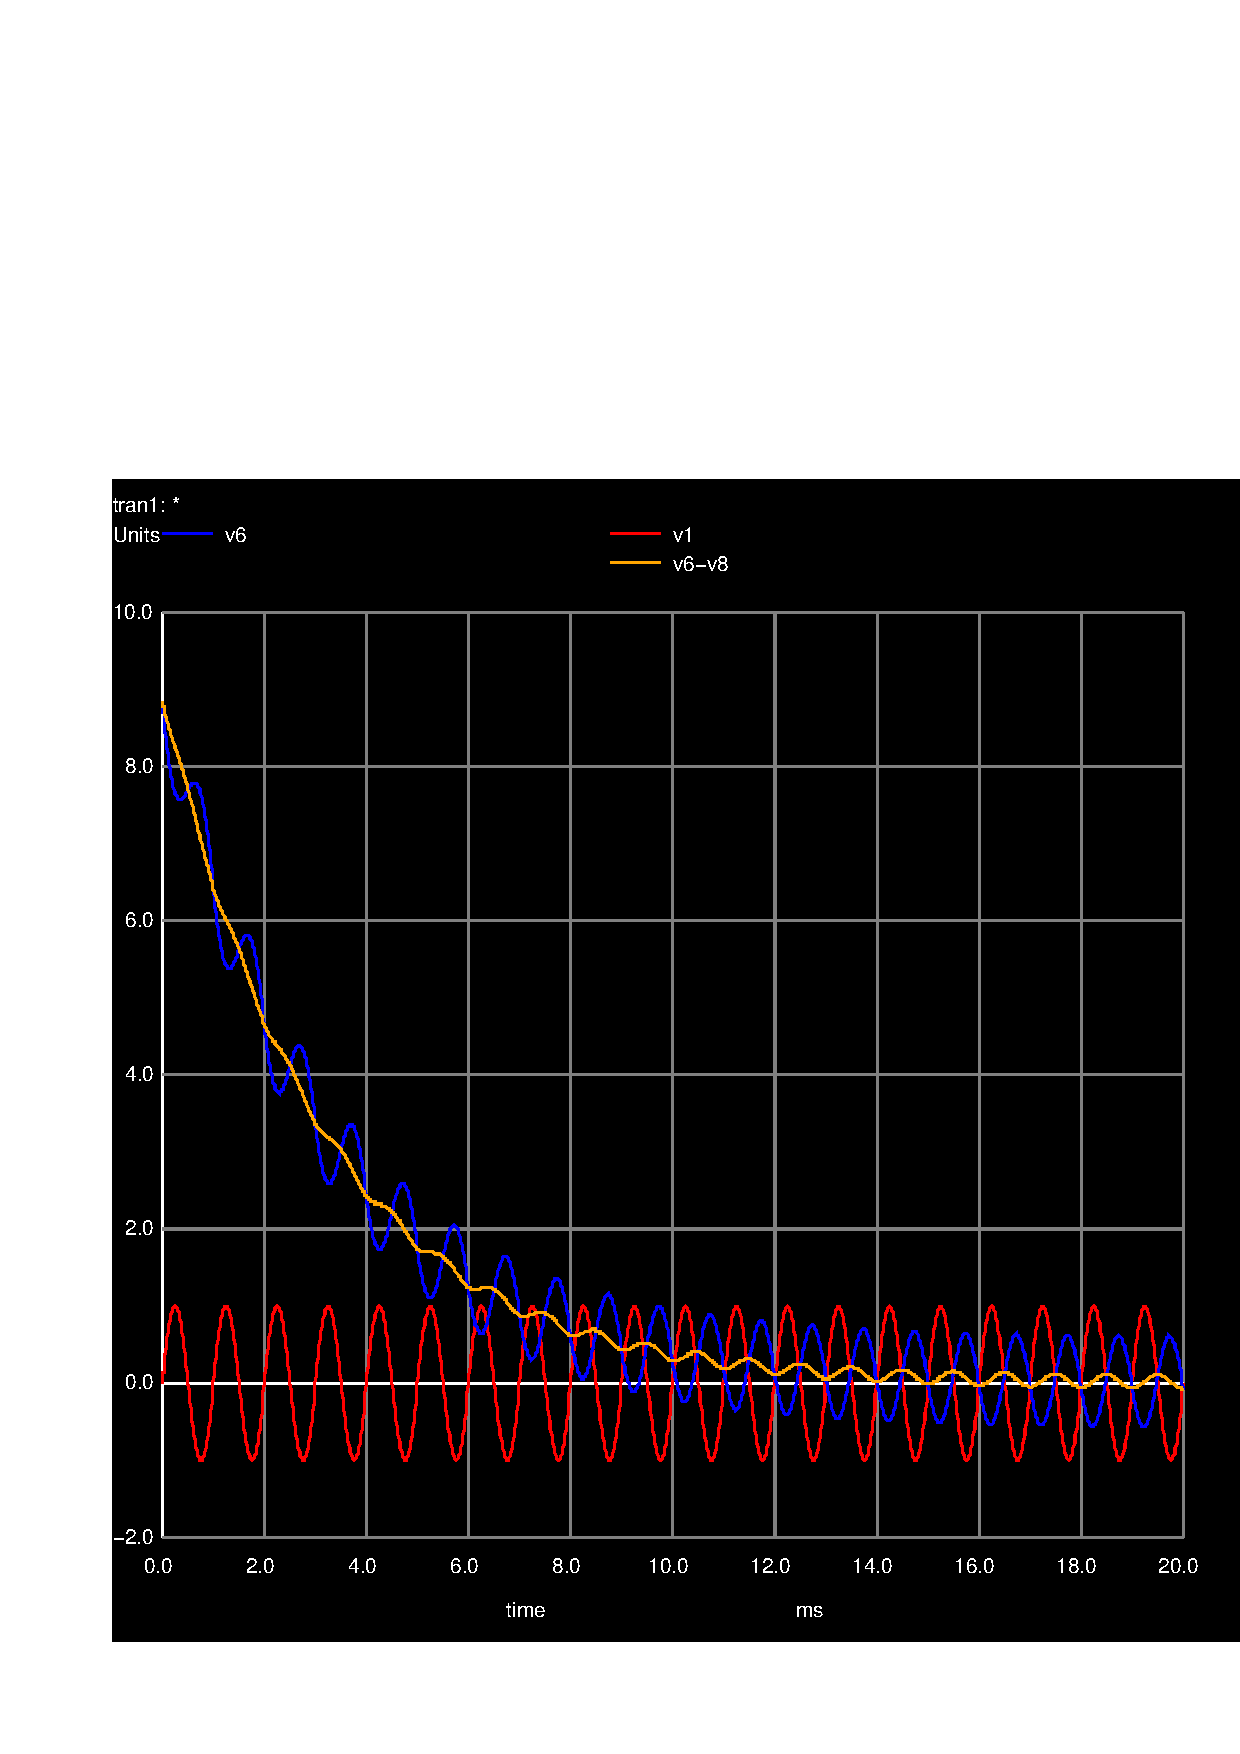
\includegraphics[width=0.4\linewidth]{trans2.pdf}
\caption{Transient output voltage for node 6, voltage source $V_s$ and capacitor $C$}
\label{fig:trans2}
\end{figure}

By analysing the result of the simulation, we notice that the total solution resulted 
of an overlap between the natural solution (in the form of a negative exponential) and
the forced solution (in a form of a sinusoidal function). Comparing to the theoretical
analysis, we notice again, because of the time interval used, the discontinuity of the 
values in t=0, that does not happen for the voltage in the capacitor. As far as the result
is concerned, the form of the theoretical solution (negative exponential+sinusoidal fuction)
match the one obtained by NGSpice.


\subsection{Frequency Analysis}

\subsubsection{Magnitude Response}

Figure~\ref{fig:acm} shows the magnitude, in decibel, of the frequency response for $v_6$, $v_s$ and the voltage in the capacitor $C$ 
of the circuit under analysis. Compared to the theoretical analysis results, we notice that we obtain the same results, 
since the graphic curves for the theoretical and simulation analysis are similar.

\begin{figure}[H] \centering
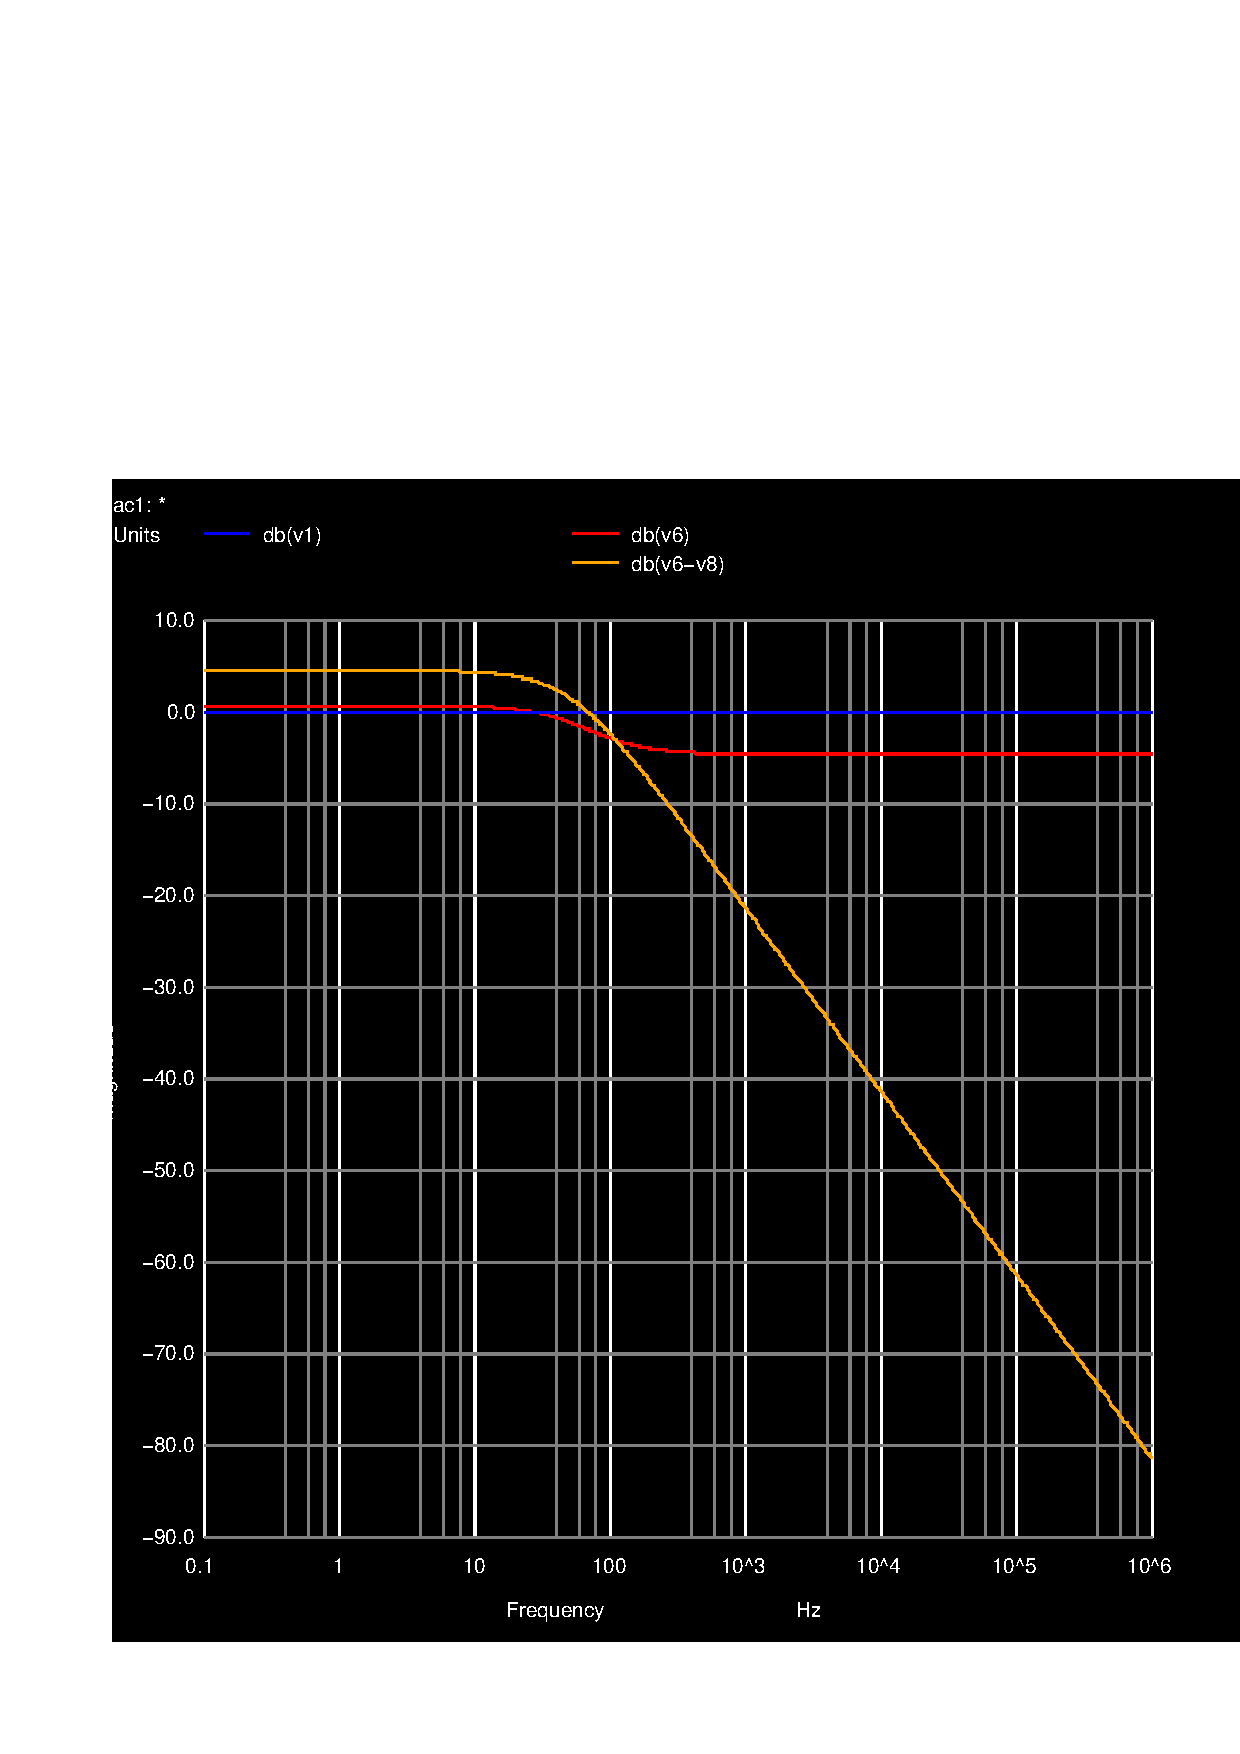
\includegraphics[width=0.4\linewidth]{acm.pdf}
\caption{Magnitude response for node 6, voltage source $V_s$ and capacitor $C$}
\label{fig:acm}
\end{figure}



\subsubsection{Phase Response}

Figure~\ref{fig:acp} shows the phase, in degrees, of the frequency response for $v_6$, $v_s$ and the voltage in the capacitor $C$ 
of the circuit under analysis. Compared to the theoretical analysis results, we notice that, again, we obtain the same results, 
since the graphic curves for the theoretical and simulation analysis are similar.

\begin{figure}[H] \centering
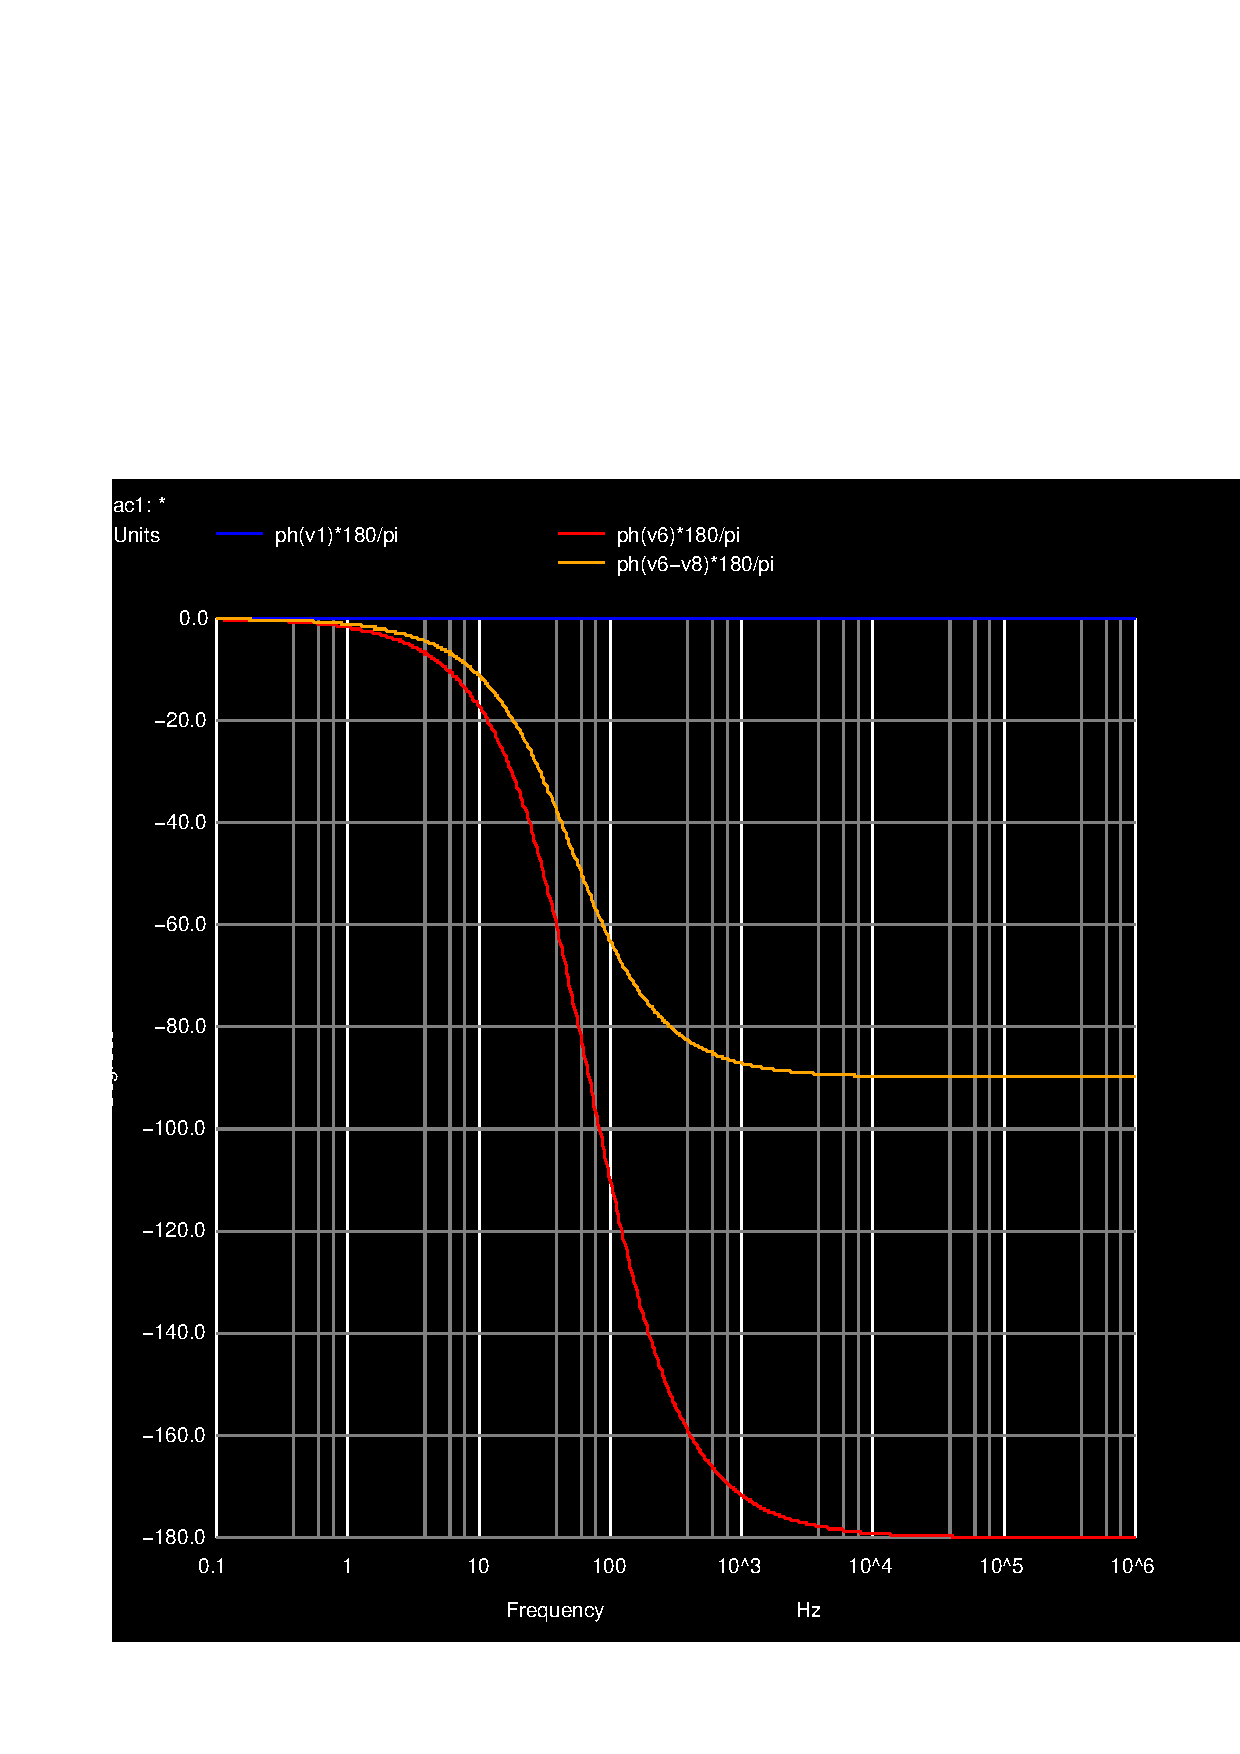
\includegraphics[width=0.4\linewidth]{acp.pdf}
\caption{Phase response for node 6, voltage source $V_s$ and capacitor $C$}
\label{fig:acp}
\end{figure}

